\documentclass[11pt]{article}
\usepackage{amssymb}
\usepackage{amsthm}
\usepackage{enumitem}
\usepackage{physics,amsmath}
\usepackage{bm}
\usepackage{adjustbox}
\usepackage{mathrsfs}
\usepackage{graphicx}
\usepackage{siunitx}
\usepackage[mathscr]{euscript}


\title{\textbf{Solved selected problems of General Relativity - Thomas A. Moore}}
\author{Franco Zacco}
\date{}

\addtolength{\topmargin}{-3cm}
\addtolength{\textheight}{3cm}

\newcommand{\hatr}{\bm{\hat{r}}}
\newcommand{\hatn}{\bm{\hat{n}}}
\newcommand{\hatx}{\bm{\hat{x}}}
\newcommand{\haty}{\bm{\hat{y}}}
\newcommand{\hatz}{\bm{\hat{z}}}
\newcommand{\hatth}{\bm{\hat{\theta}}}
\newcommand{\hatphi}{\bm{\hat{\phi}}}
\newcommand{\hatrho}{\bm{\hat{\rho}}}
\newcommand{\er}{\bm{e}_r}
\newcommand{\etht}{\bm{e}_\theta}

\theoremstyle{definition}
\newtheorem*{solution*}{Solution}
\renewcommand*{\proofname}{Solution}

\begin{document}
\maketitle
\thispagestyle{empty}

\section*{Chapter 8 - Geodesics}

\begin{proof}{\textbf{BOX 8.2} - Exercise 8.2.1.}
    Let us apply integration by parts over the last term of equation (8.25)
    which states the following
    \begin{align*}
        \int_{0}^1 \partialderivative{L}{\dot{x}^\alpha}\derivative{f^\alpha}{\sigma}~d\sigma
    \end{align*}
    Let
    \begin{align*}
        u = \partialderivative{L}{\dot{x}^\alpha}
        \quad\text{ so }\quad
        du = \derivative{}{\sigma}\bigg(\partialderivative{L}{\dot{x}^\alpha}\bigg)d\sigma
    \end{align*}
    and 
    \begin{align*}
        dv = \derivative{f^\alpha}{\sigma}d\sigma
        \quad\text{ so }\quad
        v = f^\alpha
    \end{align*}
    Then we have that
    \begin{align*}
        \int_{0}^1 \partialderivative{L}{\dot{x}^\alpha}\derivative{f^\alpha}{\sigma}~d\sigma
        &= \bigg[\partialderivative{L}{\dot{x}^\alpha}f^\alpha\bigg]_0^1
        - \int_0^1 f^\alpha \derivative{}{\sigma}\bigg(
            \partialderivative{L}{\dot{x}^\alpha}
        \bigg)d\sigma\\
        &= - \int_0^1 f^\alpha \derivative{}{\sigma}\bigg(
            \partialderivative{L}{\dot{x}^\alpha}
        \bigg)d\sigma
    \end{align*}
    Where we used that $f^\alpha(\sigma = 0) = f^\alpha(\sigma = 1) = 0$.
\end{proof}
\cleardoublepage
\begin{proof}{\textbf{BOX 8.2} - Exercise 8.2.2.}
    We know equation (8.28) is given by
    \begin{align*}
        0 = \int_{0}^1 \bigg[
            \partialderivative{L}{x^\alpha}
            - \derivative{}{\sigma}\bigg(
                \partialderivative{L}{\dot{x}^\alpha}
            \bigg)
        \bigg]f^\alpha(\sigma) d\sigma
    \end{align*}
    We want to prove that this implies that
    \begin{align*}
        \partialderivative{L}{x^\alpha}
        - \derivative{}{\sigma}\bigg(
            \partialderivative{L}{\dot{x}^\alpha}
        \bigg) = 0
    \end{align*}
    Given that $f^\alpha(\sigma)$ can be any perturbation function.
    Suppose
    \begin{align*}
        \partialderivative{L}{x^\alpha}
        - \derivative{}{\sigma}\bigg(
            \partialderivative{L}{\dot{x}^\alpha}
        \bigg) > 0
    \end{align*}
    in some interval $(c,d)$ where $0 < c < d < 1$ then if we take a "bump"
    function $f^\alpha(\sigma)$ such that it's positive on the interval $(c,d)$
    but zero elsewhere then the integrand of the equation (8.28) is positive
    and hence the integral is positive too which is a contradiction to 
    the fact that
    \begin{align*}
        \int_{0}^1 \bigg[
            \partialderivative{L}{x^\alpha}
            - \derivative{}{\sigma}\bigg(
                \partialderivative{L}{\dot{x}^\alpha}
            \bigg)
        \bigg]f^\alpha(\sigma) d\sigma = 0
    \end{align*}
    Therefore it must be that 
    \begin{align*}
        \partialderivative{L}{x^\alpha}
        - \derivative{}{\sigma}\bigg(
            \partialderivative{L}{\dot{x}^\alpha}
        \bigg) = 0
    \end{align*}
\end{proof}
\begin{proof}{\textbf{BOX 8.3} - Exercise 8.3.1.}
    Equation (8.13) states that
    \begin{align*}
        \derivative{}{\tau}\bigg(g_{\alpha\beta}\derivative{x^\beta}{\tau}\bigg)
        = \bigg(\partialderivative{g_{\alpha\beta}}{x^\gamma}
        \derivative{x^\gamma}{\tau}\bigg)\derivative{x^\beta}{\tau}
        + g_{\alpha\beta}\derivative[2]{x^\beta}{\tau}
    \end{align*}
    And equation (8.12) states that
    \begin{align*}
        0 = \derivative{}{\tau}\bigg(
        g_{\alpha\beta}\derivative{x^\beta}{\tau}\bigg)
        - \frac{1}{2}\partial_\alpha g_{\mu\nu}\derivative{x^\mu}{\tau}
        \derivative{x^\nu}{\tau}
    \end{align*}
    Let us rename $\gamma \to \mu$ and $\beta \to \nu$ on the first term
    of the equation (8.13) then
    \begin{align*}
        \derivative{}{\tau}\bigg(g_{\alpha\beta}\derivative{x^\beta}{\tau}\bigg)
        = \bigg(\partialderivative{g_{\alpha\nu}}{x^\mu}
        \derivative{x^\mu}{\tau}\bigg)\derivative{x^\nu}{\tau}
        + g_{\alpha\beta}\derivative[2]{x^\beta}{\tau}
    \end{align*}
    Now we replace this result on equation (8.12) and we multiply the equation 
    by $g^{\gamma\alpha}$ to get the equation (8.14) as follows
    \begin{align*}
        0 &= g^{\gamma\alpha}\partial_\mu g_{\alpha\nu}
        \derivative{x^\mu}{\tau}\derivative{x^\nu}{\tau}
        + g^{\gamma\alpha}g_{\alpha\beta}\derivative[2]{x^\beta}{\tau}
        - g^{\gamma\alpha}\frac{1}{2}\partial_\alpha
        g_{\mu\nu}\derivative{x^\mu}{\tau}\derivative{x^\nu}{\tau}\\
        0 &= {\delta^\gamma}_\beta\derivative[2]{x^\beta}{\tau}
        + g^{\gamma\alpha}\bigg(\partial_\mu{g_{\alpha\nu}}
        - \frac{1}{2}\partial_\alpha g_{\mu\nu}\bigg)
        \derivative{x^\mu}{\tau}\derivative{x^\nu}{\tau}\\
        0 &= \derivative[2]{x^\gamma}{\tau}
        + g^{\gamma\alpha}\bigg(\partial_\mu{g_{\alpha\nu}}
        - \frac{1}{2}\partial_\alpha g_{\mu\nu}\bigg)
        \derivative{x^\mu}{\tau}\derivative{x^\nu}{\tau}
    \end{align*}
\end{proof}
\begin{proof}{\textbf{BOX 8.4} - Exercise 8.4.1.}
    We know the geodesic equation in this case is
    \begin{align*}
        0 &= \derivative{}{s}\bigg\{
            g_{pp}\derivative{p}{s} + g_{pq}\derivative{q}{s}
        \bigg\} - \frac{1}{2}\bigg[
            \partialderivative{g_{pp}}{p} \bigg(\derivative{p}{s}\bigg)^2
            + 2 \partialderivative{g_{pq}}{p}\bigg(\derivative{p}{s}\bigg)
            \bigg(\derivative{q}{s}\bigg)
            + \partialderivative{g_{qq}}{p} \bigg(\derivative{q}{s}\bigg)^2
        \bigg]\\
        0 &= \derivative{g_{pp}}{s}\derivative{p}{s}
            + g_{pp}\derivative[2]{p}{s}
            + \derivative{g_{pq}}{s}\derivative{p}{s}
            + g_{pq}\derivative[2]{q}{s}\\
        &\quad- \frac{1}{2}\bigg[
            \partialderivative{g_{pp}}{p} \bigg(\derivative{p}{s}\bigg)^2
            + 2 \partialderivative{g_{pq}}{p}\derivative{p}{s}\derivative{q}{s}
            + \partialderivative{g_{qq}}{p} \bigg(\derivative{q}{s}\bigg)^2
        \bigg]
    \end{align*}
    Substituting the values of the metric components and their derivatives
    we get that 
    \begin{align*}
        0 &= 4c^2\derivative{p^2}{s}\derivative{p}{s}
            + [1 + 4c^2p^2]\derivative[2]{p}{s}
            + 2c\derivative{p}{s}\derivative{q}{s}
            + 2cp\derivative[2]{q}{s}\\
        &\quad- \frac{1}{2}\bigg[
            8c^2p \bigg(\derivative{p}{s}\bigg)^2
            + 4c\derivative{p}{s}
            \derivative{q}{s}
        \bigg]\\
        0 &= 8c^2p\bigg(\derivative{p}{s}\bigg)^2
            + [1 + 4c^2p^2]\derivative[2]{p}{s}
            + 2c\derivative{p}{s}\derivative{q}{s}
            + 2cp\derivative[2]{q}{s}\\
        &\quad-
            4c^2p \bigg(\derivative{p}{s}\bigg)^2
            - 2c\derivative{p}{s}\derivative{q}{s}\\
        0 &= [1 + 4c^2p^2]\derivative[2]{p}{s}
            + 4c^2p\bigg(\derivative{p}{s}\bigg)^2
            + 2cp\derivative[2]{q}{s}\\
    \end{align*}
\end{proof}
\cleardoublepage
\begin{proof}{\textbf{BOX 8.4} - Exercise 8.4.2.}
    In this case, when $\alpha = q$ the geodesic equation is
    \begin{align*}
        0 = \derivative{}{s}\bigg(
        g_{q\beta}\derivative{x^\beta}{s}\bigg)
        - \frac{1}{2}\partial_q g_{\mu\nu}\derivative{x^\mu}{s}
        \derivative{x^\nu}{s}
    \end{align*}
    Writing out the implicit sums over $\beta, \mu$ and $\nu$ gives us
    \begin{align*}
        0 = \derivative{}{s}\bigg(
            g_{qp}\derivative{p}{s} + g_{qq}\derivative{q}{s}
        \bigg)
        - \frac{1}{2}\bigg[
            \partialderivative{g_{pp}}{q} \bigg(\derivative{p}{s}\bigg)^2
            + 2 \partialderivative{g_{pq}}{q}\bigg(\derivative{p}{s}\bigg)
            \bigg(\derivative{q}{s}\bigg)
            + \partialderivative{g_{qq}}{q} \bigg(\derivative{q}{s}\bigg)^2
        \bigg]
    \end{align*}
    And substituting the values of the metric components and their derivatives
    we get that
    \begin{align*}
        0 &= 2c\derivative{p}{s}\derivative{p}{s} + 2cp\derivative[2]{p}{s}
            + \derivative[2]{q}{s}\\
        0 &= 2cp\derivative[2]{p}{s} + 2c\bigg(\derivative{p}{s}\bigg)^2
            + \derivative[2]{q}{s}
    \end{align*}
    Where we used that the partial derivatives of the metric tensor
    $g_{\alpha\beta}$ with respect to $q$ are 0.
\end{proof}
\begin{proof}{\textbf{BOX 8.4} - Exercise 8.4.3.}
    Equation (8.16) states that
    \begin{align*}
        g_{\mu\nu}\derivative{x^\mu}{s}\derivative{x^\nu}{s} = 1
    \end{align*}
    So by writing out the implicit sums over $\mu$ and $\nu$ we get that
    \begin{align*}
        g_{pp}\bigg(\derivative{p}{s}\bigg)^2
        + g_{pq}\derivative{p}{s}\derivative{q}{s}
        + g_{qp}\derivative{q}{s}\derivative{p}{s}
        + g_{qq}\bigg(\derivative{q}{s}\bigg)^2
        &= 1\\
        g_{pp}\bigg(\derivative{p}{s}\bigg)^2
        + 2g_{pq}\derivative{p}{s}\derivative{q}{s}
        + g_{qq}\bigg(\derivative{q}{s}\bigg)^2
        &= 1
    \end{align*}
    And hence by substituting values we get that
    \begin{align*}
        [1 + 4c^2(bs)^2]b^2 + 4cbs(b)(-2cb^2s + h) + 1(-2cb^2s + h)^2 &= 1\\
        b^2 + 4c^2b^4s^2 - 8c^2b^4s^2 + 4cb^2sh + 4c^2b^4s^2 - 4cb^2sh + h^2 &= 1\\
        b^2 + h^2 &= 1
    \end{align*}

\end{proof}
\cleardoublepage
\begin{proof}{\textbf{BOX 8.5} - Exercise 8.5.1.}
    In this case, when $\alpha = \theta$ the geodesic equation is
    \begin{align*}
        0 = \derivative{}{s}\bigg(
        g_{\theta\beta}\derivative{x^\beta}{s}\bigg)
        - \frac{1}{2}\partial_\theta g_{\mu\nu}\derivative{x^\mu}{s}
        \derivative{x^\nu}{s}
    \end{align*}
    Writing out the implicit sums over $\beta, \mu$ and $\nu$ gives us
    \begin{align*}
        0 &= \derivative{}{s}\bigg(
            g_{\theta\theta}\derivative{\theta}{s}
            + g_{\theta\phi}\derivative{\phi}{s}
        \bigg) -\\
        &\quad- \frac{1}{2}\bigg[
            \partialderivative{g_{\theta\theta}}{\theta}
            \bigg(\derivative{\theta}{s}\bigg)^2
            + 2 \partialderivative{g_{\theta\phi}}{\theta}
            \bigg(\derivative{\theta}{s}\bigg)
            \bigg(\derivative{\phi}{s}\bigg)
            + \partialderivative{g_{\phi\phi}}{\theta}
            \bigg(\derivative{\phi}{s}\bigg)^2
        \bigg]
    \end{align*}
    And substituting the values of the metric components and their derivatives
    we get that
    \begin{align*}
        0 &= R^2\derivative[2]{\theta}{s} - \frac{1}{2}\bigg[
            2R^2\sin\theta\cos\theta
            \bigg(\derivative{\phi}{s}\bigg)^2
        \bigg]\\
        0 &= \derivative[2]{\theta}{s} -
            \sin\theta\cos\theta
            \bigg(\derivative{\phi}{s}\bigg)^2
    \end{align*}
    On the other hand, when $\alpha = \phi$ we get that
    \begin{align*}
        0 &= \derivative{}{s}\bigg(
            g_{\phi\theta}\derivative{\theta}{s}
            + g_{\phi\phi}\derivative{\phi}{s}
        \bigg) -\\
        &\quad- \frac{1}{2}\bigg[
            \partialderivative{g_{\theta\theta}}{\phi}
            \bigg(\derivative{\theta}{s}\bigg)^2
            + 2 \partialderivative{g_{\theta\phi}}{\phi}
            \bigg(\derivative{\theta}{s}\bigg)
            \bigg(\derivative{\phi}{s}\bigg)
            + \partialderivative{g_{\phi\phi}}{\phi}
            \bigg(\derivative{\phi}{s}\bigg)^2
        \bigg]
    \end{align*}
    Again substituting the values of the metric components and their
    derivatives we get that
    \begin{align*}
        0 &= \derivative{}{s}\bigg(R^2\sin^2\theta\derivative{\phi}{s}\bigg) - 0\\
        0 &= \derivative{}{s}\bigg(\sin^2\theta\derivative{\phi}{s}\bigg)
    \end{align*}
\end{proof}
\cleardoublepage
\begin{proof}{\textbf{BOX 8.5} - Exercise 8.5.2.}
    The pathlength equation in this case is
    \begin{align*}
        1 = R^2\bigg(\derivative{\theta}{s}\bigg)^2
        + R^2\sin^2\theta\bigg(\derivative{\phi}{s}\bigg)^2
    \end{align*}
    So replacing the value for $d\phi/ds = c/R\sin^2\theta$ we have that
    \begin{align*}
        1 &= R^2\bigg(\derivative{\theta}{s}\bigg)^2
        + R^2\sin^2\theta\bigg(\frac{c}{R\sin^2\theta}\bigg)^2\\
        R^2\bigg(\derivative{\theta}{s}\bigg)^2 &= 
        1 - \frac{c^2}{\sin^2\theta}\\
        \bigg(\derivative{\theta}{s}\bigg)^2 &= 
        \frac{1}{R^2\sin^2\theta}\bigg(\sin^2\theta - c^2\bigg)\\
        \derivative{\theta}{s} &= 
        \pm\frac{1}{R\sin\theta}\sqrt{\sin^2\theta - c^2}
    \end{align*}
\end{proof}
\cleardoublepage
\begin{proof}{\textbf{BOX 8.6} - Exercise 8.6.1.}

    Let $x^\mu(\tau)$ satisfy the geodesic equation then $x^\mu(\bar{\tau})$
    also satisfy it where $\bar{\tau} = b\tau$.
    We want to prove that this doesn't happen for the equation 8.15 which
    states the following 
    \begin{align*}
        g_{\mu\nu}\derivative{x^\mu}{\tau}\derivative{x^\nu}{\tau}
        = -\bigg(\derivative{\tau}{\tau}\bigg)^2 = -1
    \end{align*}
    So using $x^\mu(\bar{\tau})$ instead of $x^\mu(\tau)$ on the left hand side
    and applying the chain rule we see that
    \begin{align*}
        g_{\mu\nu}\derivative{x^\mu(\bar\tau)}{\tau}
        \derivative{x^\nu(\bar\tau)}{\tau}
        &= g_{\mu\nu}\derivative{x^\mu(b\tau)}{\tau}
        \derivative{x^\nu(b\tau)}{\tau}
        = b^2g_{\mu\nu}\derivative{x^\mu(\bar\tau)}{\bar\tau}
        \derivative{x^\nu(\bar\tau)}{\bar\tau}
    \end{align*}
    If $x^\mu(\bar\tau)$ were to satisfy the equation 8.15 it must happen that
    \begin{align*}
        g_{\mu\nu}\derivative{x^\mu(\bar\tau)}{\bar\tau}
        \derivative{x^\nu(\bar\tau)}{\bar\tau} = -1
    \end{align*}
    But we see that instead $-1$ in this case is $-1/b^2$ 
    \begin{align*}
        g_{\mu\nu}\derivative{x^\mu(\bar\tau)}{\bar\tau}
        \derivative{x^\nu(\bar\tau)}{\bar\tau} = -\frac{1}{b^2}
    \end{align*}
    Therefore equation 8.15 is not satisfied for $\bar\tau$.
\end{proof}
\begin{proof}{\textbf{BOX 8.7} - Exercise 8.7.1.}

    For light we have that $0 = ds^2 = -dt^2 + dx^2 + dy^2 + dz^2$
    then multiplying  by $1/dt^2$ we have that
    \begin{align*}
        \bigg(\frac{dt}{dt}\bigg)^2
        &= \bigg(\frac{dx}{dt}\bigg)^2 + \bigg(\frac{dy}{dt}\bigg)^2
        + \bigg(\frac{dz}{dt}\bigg)^2\\
        1 &= (v^x)^2 + (v^y)^2 + (v^z)^2\\
        1 &= v^2
    \end{align*}
    Therefore the velocity of light is $v = 1$.
\end{proof}
\cleardoublepage
\begin{proof}{\textbf{P8.1}}
\begin{itemize}
    \item [\textbf{a.}]
    We know that if light is emitted at a distance $z$ from the earth $z=0$
    then the light is blue-shifted as follows
    \begin{align*}
        \frac{\lambda}{\lambda_e} = 1 - gz
    \end{align*}
    so if we consider the time between two succesive crests of the light wave
    as they are emitted to be an infinitesimal coordinate time $dt$ for
    the observer at $z=0$ and $dT$ for the observer at a higher position
    $z$ then we have that $\lambda = c dt$ and $\lambda_e = c dT$
    so by replacing this values we have that
    \begin{align*}
        1 - gz &= \frac{cdt}{cdT}\\
        (1 - gz)dT &= dt\\
        dT &= \frac{dt}{1 - gz}
    \end{align*}
    Finally, since $gz \ll 1$ we can apply the binomial approximation to
    $(1 - gz)^{-1}$ to get that
    \begin{align*}
        dT \approx (1 + gz)dt
    \end{align*}
    \item [\textbf{b.}]
    The proper time $d\tau$ that the projectile clock reads between two
    infinitesimally separated events at $z$ due to time dilation is
    \begin{align*}
        d\tau = \sqrt{1 - v^2} dT
    \end{align*}
    where $dT$ is the time measured by a clock at $z$, again assuming $v \ll 1$
    by the binomial approximation we have that
    \begin{align*}
        d\tau \approx \bigg(1 - \frac{1}{2}v^2\bigg) dT
    \end{align*}
    But we know that $dT$ is related to the time $dt$ read by an observer at
    $z=0$ by $dT = (1 + gz)dt$ so $d\tau$ and $dt$ are related by
    \begin{align*}
        d\tau &= \bigg(1 - \frac{1}{2}v^2\bigg) (1 + gz) dt\\
        d\tau &= \bigg(1 + gz -\frac{1}{2}v^2 - \frac{1}{2}v^2 gz\bigg) dt\\
        d\tau &\approx \bigg(1 + gz -\frac{1}{2}v^2\bigg) dt
    \end{align*}
    where in the last step we removed the term $1/2v^2 gz$ since we are
    assuming $v \ll 1$ and $gz \ll 1$ therefore the term is insignificant.
    \item [\textbf{c.}]
    Let us define a Lagrangian
    $L = 1 - \frac{1}{2}(\dot x^2 + \dot y^2 + \dot z^2) + gz$
    we want to maximize the equation
    \begin{align*}
        \tau_B - \tau_A = \int_{t_A}^{t_B} L~dt
    \end{align*}
    We know that the trajectory that maximizes this equation must also satisfy
    the Euler-Lagrange equations
    \begin{align*}
        0 = \derivative{}{t}\bigg(\partialderivative{L}{\dot x^\mu}\bigg)
        - \partialderivative{L}{x^\mu}
    \end{align*}
    Hence for $x$ and $y$ this equation becomes $\ddot x = 0$ and $\ddot y = 0$
    but for $z$ this gives us 
    \begin{align*}
        0 &= \derivative{}{t}\bigg(\partialderivative{L}{\dot z}\bigg)
        - \partialderivative{L}{z}\\
        0 &= \ddot z - g
    \end{align*}
    Below we solve the differential equation for $x$ but the same applies to
    the equation for $y$ which give us $y = v_0 t + y_0$.
    \begin{align*}
        \derivative{v_x}{t} &= 0\\
        \derivative{x}{t} - v_0 &= 0\\
        x &= v_0t + x_0
    \end{align*}
    Finally, for $z$ we have that
    \begin{align*}
        \derivative{v_z}{t} &= g\\
        \derivative{z}{t} &= gt + v_0\\
        z &= \frac{1}{2}gt^2 + v_0 t + z_0
    \end{align*}
    Therefore we got the standard parabola equations we were expecting.
\end{itemize}
\end{proof}
\cleardoublepage
\begin{proof}{\textbf{P8.2}}
    \begin{itemize}
        \item [\textbf{a.}] Equation 8.46 states the following
        \begin{align*}
            \derivative{\theta}{s}
            = \pm \frac{1}{R\sin\theta}\sqrt{\sin^2\theta - c^2}
        \end{align*}
        Then we can rearrange it as follows
        \begin{align*}
            ds\sqrt{\sin^2\theta - c^2} &= d\theta R\sin\theta\\
            ds &= \frac{R\sin\theta d\theta}{\sqrt{\sin^2\theta - c^2}}
        \end{align*}
        Finally, if we define $a^2 = 1 - c^2$ and we recall that
        $\sin^2\theta = 1 - \cos^2\theta$ we get that
        \begin{align*}
            ds &= \frac{R\sin\theta d\theta}{\sqrt{1 -\cos^2\theta - c^2}}\\
            ds &= \frac{R\sin\theta d\theta}{\sqrt{a^2 -\cos^2\theta}}
        \end{align*}
        \item [\textbf{b.}] Let $u = \cos\theta$ then $du = -\sin\theta d\theta$ then we have that
        \begin{align*}
            ds &= -\frac{Rdu}{\sqrt{a^2 -u^2}}
        \end{align*}
        By integration we have that
        \begin{align*}
            \int ds &= -R\int \frac{du}{\sqrt{a^2 -u^2}}\\
            s &= -R \arcsin\bigg(\frac{u}{a}\bigg) + C
        \end{align*}
        Where $C$ is a constant of integration which is equal to 0 since the
        intial conditions of $s = 0$ when $u = 0$ gives us $C = 0$.
        So we get that 
        \begin{align*}
            \cos\theta = u &= \pm a\sin\bigg(\frac{s}{R}\bigg) = \pm a\sin\psi
        \end{align*}
        Where we defined $\psi = s/R$.

        \item [\textbf{c.}]
        Equation 8.43 states that
        \begin{align*}
            \derivative{\phi}{s} = \frac{c}{R\sin^2\theta}
        \end{align*}
        Replacing that $\sin^2\theta = 1 - \cos^2\theta = 1 - a^2\sin^2\psi$
        we get that
        \begin{align*}
            \derivative{\phi}{s} = \frac{c}{R(1 - a^2 \sin^2\psi)}
        \end{align*}
        Also, we know from part \textbf{b.} that $\psi = s/R$ hence $d\psi = ds/R$ so replacing this and integrating both sides we get that
        \begin{align*}
            \int d\phi &= c\int \frac{d\psi}{(1 - a^2 \sin^2\psi)}\\
            \phi - \phi_0 &= \frac{c\arctan(\sqrt{1 - a^2} \tan(\psi))}{\sqrt{1 - a^2}}\\
            \phi - \phi_0 &= \arctan(c \tan(\psi))\\
            \tan(\phi - \phi_0) &= c \tan(\psi)
        \end{align*}
        Where we used that $c = \sqrt{1 - a^2}$.

        \item [\textbf{d.}] Replacing $z = my$ into the equation for the
        surface of a sphere, we get that
        \begin{align*}
            x^2 + y^2 + m^2y^2 = R
        \end{align*}
        And using the definitions $x = R\sin\theta\cos\phi$ and
        $y=R\sin\theta\sin\phi$ in spherical coordinates we get that
        \begin{align*}
            (R\sin\theta\cos\phi)^2 + (R\sin\theta\sin\phi)^2(1 + m^2) &= R\\
            (\sin\theta\cos\phi)^2 + (\sin\theta\sin\phi)^2(1 + m^2) &= 1\\
            \sin^2\theta(\cos^2\phi + \sin^2\phi) + m^2\sin^2\theta\sin^2\phi &= 1\\
            \sin^2\theta(1 + m^2\sin^2\phi) &= 1\\
            m^2\sin^2\phi &= \frac{1}{\sin^2\theta} -1\\
            m\sin\phi &= \sqrt{\frac{1}{\sin^2\theta} -1} = \cot\theta
        \end{align*}

        \item [\textbf{e.}] Let us note first that
        $\sin\phi = \tan\phi /\sqrt{1 + \tan^2\phi}$ so using this equation
        and the equation we got from part \textbf{c.} assuming $\phi_0 = 0$
        we get that
        \begin{align*}
            \sin(\phi) &= \frac{c\tan\psi}{\sqrt{1 + c^2\tan^2\psi}}
        \end{align*}
        If we divide and multiply by $\cos\psi$ we get that
        \begin{align*}
            \sin\phi &= \frac{c\tan\psi\cos\psi}{\cos\psi\sqrt{1 + c^2\tan^2\psi}}\\
            \sin\phi &= \frac{c\sin\psi}{\sqrt{\cos^2\psi + c^2\sin^2\psi}}\\
            \sin\phi &= \frac{c\sin\psi}{\sqrt{\cos^2\psi + (1 - a^2)\sin^2\psi}}\\
            \sin\phi &= \frac{c\sin\psi}{\sqrt{1 - a^2\sin^2\psi}}
        \end{align*}
        Finally, using equations 8.53 and 8.54 we have that
        \begin{align*}
            \sin\phi &= \frac{c\cos\theta}{a\sin\theta}\\
            \frac{a}{c}\sin\phi &= \cot\theta
        \end{align*}
        Which is the great circle equation we wanted.
    \end{itemize}
\end{proof}
\cleardoublepage
\begin{proof}{\textbf{P8.3}}
    \begin{itemize}
        \item [\textbf{a.}] By the right triangle $OBP$ the length of the
        hypotenuse $r$ is given by
        \begin{align*}
            r^2 = s^2 + b^2
        \end{align*}
        and the angle $\theta$ between $r$ and the $x$ axis is given by
        the sum of $\alpha$ and the angle between $b$ and $r$ which is 
        $\arctan(s/b)$ hence
        \begin{align*}
            \theta = \alpha + \arctan(\frac{s}{b})
        \end{align*}
        So for any value of $s$ the points determined by these equations must
        be on the line in question.
        
        \item [\textbf{b.}] Knowing that the polar coordinates metric is
        \begin{align*}
            g_{\mu\nu} = \begin{bmatrix}
                1 & 0 \\ 0 & r^2
            \end{bmatrix}
        \end{align*}
        We can compute the geodesic equation for $\alpha = r$ as follows
        \begin{align*}
            0 &= \derivative{}{s}\bigg(
            g_{r\beta}\derivative{x^\beta}{s}\bigg)
            - \frac{1}{2}\partial_r g_{\mu\nu}\derivative{x^\mu}{s}
            \derivative{x^\nu}{s}\\
            0 &= \derivative{}{s}\bigg(
            \derivative{r}{s}\bigg)
            - \frac{1}{2}(2r)\bigg(\derivative{\theta}{s}\bigg)^2\\
            \derivative[2]{r}{s} &= r\bigg(\derivative{\theta}{s}\bigg)^2
        \end{align*}
        and for $\alpha = \theta$ we have that
        \begin{align*}
            0 &= \derivative{}{s}\bigg(
            g_{\theta\beta}\derivative{x^\beta}{s}\bigg)
            - \frac{1}{2}\partial_\theta g_{\mu\nu}\derivative{x^\mu}{s}
            \derivative{x^\nu}{s}\\
            0 &= \derivative{}{s}\bigg(r^2\derivative{\theta}{s}\bigg) + 0\\
            \derivative{\theta}{s} &= \frac{c}{r^2}
        \end{align*}
        Where in the last step we integrated the expression with respect to $s$
        and $c$ is a constant of integration.
        Now replacing the value for $d\theta/ds$ on the geodesic
        for $\alpha = r$ we get that
        \begin{align*}
            \derivative[2]{r}{s} &= \frac{c^2}{r^3}
        \end{align*}

        \item [\textbf{c.}] The pathlength equation states that
        \begin{align*}
            g_{\mu\nu}\derivative{x^\mu}{s}\derivative{x^\nu}{s} = 1
        \end{align*}
        So applied to this case we get that
        \begin{align*}
            \bigg(\derivative{r}{s}\bigg)^2
            + r^2\bigg(\derivative{\theta}{s}\bigg)^2 = 1
        \end{align*}
        So replacing the value of $d\theta/ds$ from equation (8.62) we have that
        \begin{align*}
            \derivative{r}{s}
            &= \sqrt{1 - r^2\bigg(\derivative{\theta}{s}\bigg)^2}\\
            &= \sqrt{1 - \frac{c^2}{r^2}}
        \end{align*}

        \item [\textbf{d.}] Derivating equation (8.64) on both sides we get that
        \begin{align*}
            \derivative{}{s}\bigg(\derivative{r}{s}\bigg)
            &= \derivative{}{s}\bigg(\sqrt{1 - \frac{c^2}{r^2}}\bigg)\\
            \derivative[2]{r}{s}
            &= \frac{c^2~dr/ds}{r^3\sqrt{1 - \frac{c^2}{r^2}}}\\
            \derivative[2]{r}{s} &= \frac{c^2}{r^3}
        \end{align*}

        \item [\textbf{e.}] From equation (8.64) we have that 
        \begin{align*}
            \derivative{r}{s} &= \sqrt{1 - \frac{c^2}{r^2}}\\
            \int \frac{dr}{\sqrt{1 - \frac{c^2}{r^2}}} &= \int ds\\
            \sqrt{r^2 - c^2} &= s\\
            r^2 &= s^2 + c^2
        \end{align*}

        \item [\textbf{f.}] Replacing $r^2 = s^2 + c^2$ on equation (8.62)
        assuming $c = b$ we get that
        \begin{align*}
            \derivative{\theta}{s} &= \frac{b}{r^2}\\
            \derivative{\theta}{s} &= \frac{b}{s^2 + b^2}\\
            \int d\theta &= b\int \frac{ds}{s^2 + b^2}\\
            \theta &= \arctan(\frac{s}{\sqrt{s^2 + b^2}}) + \alpha\\
            \theta &= \arctan(\frac{s}{r}) + \alpha
        \end{align*}
        Where $\alpha$ is some constant of integration.
    \end{itemize}
\end{proof}
\begin{proof}{\textbf{P8.4}}
    \begin{itemize}
        \item [\textbf{a.}] We know that the geodesic equation is
        \begin{align*}
            0 &= \derivative{}{\tau}\bigg(
            g_{\alpha\beta}\derivative{x^\beta}{\tau}\bigg)
            - \frac{1}{2}\partial_\alpha g_{\mu\nu}\derivative{x^\mu}{\tau}
            \derivative{x^\nu}{\tau}\\
            0 &= \derivative{}{\tau}\big(g_{\alpha\beta}u^\beta\big)
            - \frac{1}{2}\partial_\alpha g_{\mu\nu}u^\mu u^\nu
        \end{align*}
        Then by the product rule we have that
        \begin{align*}
            0 &=
            \bigg(g_{\alpha\beta}\derivative{u^\beta}{\tau}
            + \derivative{g_{\alpha\beta}}{\tau}u^\beta\bigg) 
            - \frac{1}{2}\partial_\alpha g_{\mu\nu}u^\mu u^\nu\\
            0 &=
            g_{\alpha\beta}\derivative{u^\beta}{\tau}
            + \derivative{g_{\alpha\beta}}{\tau}
            \derivative{x^\sigma}{x^\sigma}u^\beta  
            - \frac{1}{2}\partial_\alpha g_{\mu\nu}u^\mu u^\nu\\
            0 &=
            g_{\alpha\beta}\derivative{u^\beta}{\tau}
            + \derivative{g_{\alpha\beta}}{x^\sigma}
            \derivative{x^\sigma}{\tau}u^\beta  
            - \frac{1}{2}\partial_\alpha g_{\mu\nu}u^\mu u^\nu\\
            0 &=
            g_{\alpha\beta}\derivative{u^\beta}{\tau}
            + \partial_\sigma g_{\alpha\beta}
            u^\sigma u^\beta  
            - \frac{1}{2}\partial_\alpha g_{\mu\nu}u^\mu u^\nu
        \end{align*}
        \item [\textbf{b.}] We want to prove now that $\bm{u}\cdot\bm{u}$
        is constant for any object following a geodesic.
        Let us compute $d(\bm{u}\cdot\bm{u}) /d\tau$
        \begin{align*}
            \derivative{\bm{u}\cdot\bm{u}}{\tau}
            &= \derivative{}{\tau}\bigg(
                g_{\mu\nu}\derivative{x^\mu}{\tau}\derivative{x^\nu}{\tau}
            \bigg)\\
            &=
            \derivative{g_{\mu\nu}}{\tau}\derivative{x^\mu}{\tau}
            \derivative{x^\nu}{\tau}
            + g_{\mu\nu}\derivative{}{\tau}\bigg(\derivative{x^\mu}{\tau}
            \derivative{x^\nu}{\tau}\bigg)\\
            &=
            \derivative{g_{\mu\nu}}{\tau}\derivative{x^\mu}{\tau}
            \derivative{x^\nu}{\tau}
            + g_{\mu\nu}\derivative[2]{x^\mu}{\tau}
            \derivative{x^\nu}{\tau}
            + g_{\mu\nu}\derivative{x^\mu}{\tau}
            \derivative[2]{x^\nu}{\tau}\\
            &=
            \partial_\sigma g_{\mu\nu} u^\sigma u^\mu u^\nu
            + g_{\mu\nu}\derivative{u^\mu}{\tau}u^\nu
            + g_{\mu\nu}u^\mu\derivative{u^\nu}{\tau}\\
            &=
            \partial_\sigma g_{\mu\nu} u^\sigma u^\mu u^\nu
            + 2g_{\mu\nu}\derivative{u^\mu}{\tau}u^\nu
        \end{align*}
        Where we used that $g_{\mu\nu} = g_{\nu\mu}$ to sum the last two terms.
        Also, multiplying equation (8.65) by $u^\alpha$ we get that
        \begin{align*}
            0 &=
            g_{\alpha\beta}u^\alpha\derivative{u^\beta}{\tau}
            + \partial_\sigma g_{\alpha\beta} u^\alpha u^\beta u^\sigma  
            - \frac{1}{2}\partial_\alpha g_{\mu\nu}u^\mu u^\nu u^\alpha\\
            0 &=
            g_{\alpha\beta}u^\alpha\derivative{u^\beta}{\tau}
            + \frac{1}{2}\partial_\sigma g_{\alpha\beta} u^\alpha u^\beta u^\sigma\\
            0 &=
            2g_{\beta\alpha}\derivative{u^\beta}{\tau}u^\alpha
            + \partial_\sigma g_{\alpha\beta} u^\sigma u^\alpha u^\beta
        \end{align*}
        Where we subtracted the last two terms since they differ only in the
        names of the subscripts and superscripts and we multiplied the whole
        equation by 2.
        
        Finally, comparing both equations we see that they are the same
        equation but with different variable namings, so this implies that
        $d(\bm{u}\cdot\bm{u})/d\tau = 0$ and therefore that $\bm{u}\cdot\bm{u}$
        is constant.
    \end{itemize}
\end{proof}
\begin{proof}{\textbf{P8.5}}
    \begin{itemize}
        \item [\textbf{a.}] In this case the metric is given by
        \begin{align*}
            g_{\mu\nu} = \begin{bmatrix}
                -1 & 0 \\
                0 & f(q)^2
            \end{bmatrix}
        \end{align*}
        So the geodesic equations are
        \begin{align*}
            0 &= \derivative{}{\tau}\bigg(
            g_{t\beta}\derivative{x^\beta}{\tau}\bigg)
            - \frac{1}{2}\partial_t g_{\mu\nu}\derivative{x^\mu}{\tau}
            \derivative{x^\nu}{\tau}\\
            0 &= -\derivative[2]{t}{\tau}
        \end{align*}
        And when $\alpha = q$ we have that
        \begin{align*}
            0 &= \derivative{}{\tau}\bigg(
            g_{q\beta}\derivative{x^\beta}{\tau}\bigg)
            - \frac{1}{2}\partial_q g_{\mu\nu}\derivative{x^\mu}{\tau}
            \derivative{x^\nu}{\tau}\\
            0 &= \derivative{}{\tau}\bigg(
            f(q)^2\derivative{q}{\tau}\bigg)
            - \frac{1}{2}\derivative{f(q)^2}{q}\bigg(\derivative{q}{\tau}\bigg)^2\\
            0 &= \derivative{f(q)^2}{\tau}\derivative{q}{\tau}
            + f(q)^2\derivative[2]{q}{\tau}
            - f(q)\derivative{f(q)}{q}\bigg(\derivative{q}{\tau}\bigg)^2\\
            0 &= 2f(q)\derivative{f(q)}{q}\bigg(\derivative{q}{\tau}\bigg)^2
            + f(q)^2\derivative[2]{q}{\tau}
            - f(q)\derivative{f(q)}{q}\bigg(\derivative{q}{\tau}\bigg)^2\\
            0 &= f(q)\derivative{f(q)}{q}\bigg(\derivative{q}{\tau}\bigg)^2
            + f(q)^2\derivative[2]{q}{\tau}
        \end{align*}
        So from the first equation we see that $dt/d\tau = c$ where $c$ is
        a constant.

        \item[\textbf{b.}] Let $\bm{u}\cdot\bm{u} = -1$ then we have that
        \begin{align*}
            g_{\mu\nu}\derivative{x^\mu}{\tau}\derivative{x^\nu}{\tau} &= -1\\
            -\bigg(\derivative{t}{\tau}\bigg)^2
            + f(q)^2\bigg(\derivative{q}{\tau}\bigg)^2 &= -1\\
            f(q)\derivative{q}{\tau}
            &= \sqrt{\bigg(\derivative{t}{\tau}\bigg)^2 - 1}
        \end{align*}
        And since $dt/d\tau$ is constant then $fdq/d\tau$ is a constant too.

        \item[\textbf{c.}] Since $fdq/d\tau$ is a constant then we can write
        that
        \begin{align*}
            f\derivative{q}{\tau}\derivative{t}{t} &= c_1\\
            f\derivative{q}{t}\derivative{t}{\tau} &= c_1\\
            f\derivative{q}{t}c_2 &= c_1\\
            \derivative{q}{t} &= \frac{c}{f}
        \end{align*}
        Where we define the constant $c$ as $c = c_1/c_2$.

        \item[\textbf{d.}] We can compute the metric in the new coordinate
        system from the flat metric $g_{\alpha\beta}$ with the following
        equation
        \begin{align*}
            g'_{\mu\nu} = \partialderivative{x^\alpha}{x'^\mu}
            \partialderivative{x^\beta}{x'^\nu}g_{\alpha\beta}
        \end{align*}
        Hence
        \begin{align*}
            g'_{tt} &= \partialderivative{t}{t}
            \partialderivative{t}{t}g_{tt}
            + \partialderivative{t}{t}
            \partialderivative{x}{t}g_{tx}
            + \partialderivative{x}{t}
            \partialderivative{t}{t}g_{xt}
            + \partialderivative{x}{t}
            \partialderivative{x}{t}g_{xx}\\
            &= -\bigg(\partialderivative{t}{t}\bigg)^2
            + \bigg(\partialderivative{x}{t}\bigg)^2\\
            &= -1
            + \bigg(\partialderivative{F(q)}{t}\bigg)^2\\
            &= -1\\
            g'_{tq} &= \partialderivative{t}{t}
            \partialderivative{t}{q}g_{tt}
            + \partialderivative{t}{t}
            \partialderivative{x}{q}g_{tx}
            + \partialderivative{x}{t}
            \partialderivative{t}{q}g_{xt}
            + \partialderivative{x}{t}
            \partialderivative{x}{q}g_{xx}
            = 0\\
            g'_{qt} &= \partialderivative{t}{q}
            \partialderivative{t}{t}g_{tt}
            + \partialderivative{t}{q}
            \partialderivative{x}{t}g_{tx}
            + \partialderivative{x}{q}
            \partialderivative{t}{t}g_{xt}
            + \partialderivative{x}{q}
            \partialderivative{x}{t}g_{xx}
            = 0\\
            g'_{qq} &= \partialderivative{t}{q}
            \partialderivative{t}{q}g_{tt}
            + \partialderivative{t}{q}
            \partialderivative{x}{q}g_{tx}
            + \partialderivative{x}{q}
            \partialderivative{t}{q}g_{xt}
            + \partialderivative{x}{q}
            \partialderivative{x}{q}g_{xx}\\
            &= \bigg(\partialderivative{x}{q}\bigg)^2\\
            &= \bigg(\partialderivative{F(q)}{q}\bigg)^2\\
            &= f(q)^2
        \end{align*}
        Where we used that $dF(q)/dq = f(q)$ since $F(q)$ is the antiderivative
        of $f(q)$.
        
        Therefore the metric $ds^2 = -dt^2 + f(q)^2dq^2$ is actually the metric
        for flat spacetime in disguise.         
    \end{itemize}
\end{proof}
\begin{proof}{\textbf{P8.6}}
    Let us consider a 2D spacetime whose metric is
    \begin{align*}
        ds^2 = -e^{-x/a}dt^2 + dx^2
    \end{align*}
    \begin{itemize}
        \item [\textbf{a.}] The geodesic equations when $\alpha = t$ gives us
        \begin{align*}
            0 &= \derivative{}{\tau}\bigg(
            g_{t\beta}\derivative{x^\beta}{\tau}\bigg)
            - \frac{1}{2}\partial_t g_{\mu\nu}\derivative{x^\mu}{\tau}
            \derivative{x^\nu}{\tau}\\
            0 &= \derivative{}{\tau}\bigg(
                -e^{-x/a}\derivative{t}{\tau}\bigg)
                - \frac{1}{2} \bigg(
                0\cdot\derivative[2]{t}{\tau}
                + 0\cdot\derivative[2]{x}{\tau}
            \bigg)\\
            0 &= \derivative{}{\tau}\bigg(-e^{-x/a}\derivative{t}{\tau}\bigg)
        \end{align*}
        By integration on both sides with respect to $d\tau$ we see that
        \begin{align*}
            -e^{-x/a}\derivative{t}{\tau} &= c\\
            \derivative{t}{\tau} &= ce^{x/a}
        \end{align*}
        Where $c$ is some constant.

        \item [\textbf{b.}] If we require that $\bm{u\cdot u} = -1$ we get that
        \begin{align*}
            g_{\mu\nu}\derivative{x^\mu}{\tau}\derivative{x^\nu}{\tau} &= -1\\
            -e^{-x/a}\bigg(\derivative{t}{\tau}\bigg)^2
            + \bigg(\derivative{x}{\tau}\bigg)^2 &= -1\\
            \derivative{x}{\tau}
            &= \pm\sqrt{e^{-x/a}\bigg(\derivative{t}{\tau}\bigg)^2 - 1}\\
            \derivative{x}{\tau}
            &= \pm\sqrt{e^{-x/a}\bigg(c e^{x/a}\bigg)^2 - 1}\\
            \derivative{x}{\tau}
            &= \pm\sqrt{c^2 e^{x/a} - 1}
        \end{align*}
        Where we used the value we computed before for $dt/d\tau$.
        
        \item [\textbf{c.}] Let's compute $dx/dt = (dx/d\tau)/(dt/d\tau)$ as
        follows
        \begin{align*}
            \derivative{x}{t} &= \frac{\sqrt{c^2 e^{x/a} - 1}}{ce^{x/a}}\\
            \int_0^t dt &= \int_{x_0}^x \frac{ce^{x/a}~dx}{\sqrt{c^2 e^{x/a} - 1}}\\
            t &= \bigg[\frac{2a}{c}\sqrt{c^2 e^{x/a} - 1}\bigg]_{x_0}^x\\
            t &= \frac{2a}{c}
            \bigg(\sqrt{c^2 e^{x/a} - 1} - \sqrt{c^2 e^{x_0/a} - 1}\bigg)
        \end{align*}
        Now inverting this equation to get $x(t)$ we have that
        \begin{align*}
            \sqrt{c^2 e^{x/a} - 1}
            &= \frac{tc}{2a} + \sqrt{c^2 e^{x_0/a} - 1}\\
            c^2 e^{x/a} &= \bigg(\frac{tc}{2a}
            + \derivative{x}{\tau}\bigg|_{x_0}\bigg)^2 + 1\\
            e^{x/a} &=
            \bigg(\frac{t}{2a} + \frac{u_0}{c}\bigg)^2 + \frac{1}{c^2}\\
            x &= a\ln\bigg[\bigg(\frac{t}{2a} + \frac{u_0}{c}\bigg)^2
            + \frac{1}{c^2}\bigg]
        \end{align*}
        We see that when $t=0$ we have that
        \begin{align*}
            x(0) &= a\ln\bigg[\bigg(\frac{u_0}{c}\bigg)^2
            + \frac{1}{c^2}\bigg]\\
            &= a\ln\bigg[\frac{c^2 e^{x_0/a} - 1}{c^2}
            + \frac{1}{c^2}\bigg]\\
            &= a\ln\bigg[e^{x_0/a}-\frac{1}{c^2} + \frac{1}{c^2}\bigg]\\
            &= a\ln\bigg[e^{x_0/a}\bigg]\\
            &= x_0
        \end{align*}

        \item [\textbf{d.}] If $x_0 = 0$ and $u_0 = 0$ then the constant $c$
        is
        \begin{align*}
            a\ln\bigg[\frac{1}{c^2}\bigg] &= 0\\
            \frac{1}{c^2} &= 1\\
            c &= \pm 1
        \end{align*}
        So the trajectory of the particle is given by
        \begin{align*}
            \frac{x}{a} &= \ln\bigg[\bigg(\frac{t}{2a}\bigg)^2 + 1\bigg]
        \end{align*}
\cleardoublepage
        And the graph for this geodesic is shown below
        \begin{center}
            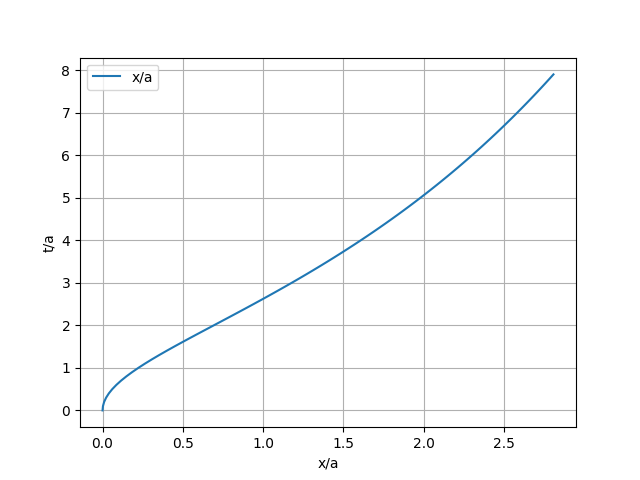
\includegraphics[scale=0.8]{ch8-6.png}
        \end{center}

        \item [\textbf{e.}] We want to find expressions for $x(\tau)$ and
        $t(\tau)$ where we set that $x=0$ and $t=0$ when $\tau = 0$.
        We know from part (d) that $c = 1$ and we have an expression for $x/a$
        so we can integrate the equations we got from part (a)
        as follows
        \begin{align*}
            \derivative{t}{\tau} &= e^{x/a}\\
            \derivative{t}{\tau} &= \bigg(\frac{t}{2a}\bigg)^2 + 1\\
            \int_{0}^t \frac{dt}{t^2/4a^2  + 1} &= \int_0^\tau d\tau\\
            \frac{2}{a}\arctan(\frac{at}{2}) &= \tau\\
            t &= \frac{2}{a}\tan(\frac{a\tau}{2})
        \end{align*}
        And for $dx/d\tau$ we have that
        \begin{align*}
            \derivative{x}{\tau} &= \sqrt{e^{x/a} - 1}\\
            \int_{0}^x \frac{dx}{\sqrt{e^{x/a} - 1}} &= \int_0^\tau d\tau\\
            2a\arctan(\sqrt{e^{x/a} - 1}) &= \tau\\
            e^{x/a} &= \tan^2\bigg(\frac{\tau}{2a}\bigg) + 1\\
            x &= a\ln(\tan^2\bigg(\frac{\tau}{2a}\bigg) + 1)
        \end{align*}
        Let us consider the equation we got for $\tau$ when we integrated over
        $t$ given by
        \begin{align*}
            \tau &= \frac{2}{a}\arctan(\frac{at}{2})
        \end{align*}
        Since $\tau$ is an arctan function of $t$ then as $t \to \infty$,
        $\tau$ approaches a maximum which is given by
        \begin{align*}
            \tau_{max} = \frac{\pi}{a} 
        \end{align*}
        Since $\arctan(at/2) \to \pi/2$ as $t \to \infty$.
    \end{itemize}
\end{proof}
\cleardoublepage
\begin{proof}{\textbf{P8.7}}
    \begin{itemize}
        \item [\textbf{a.}] To determine the distance of infinitesimally
        separated points $ds^2$ on the surface we need to consider first an
        infinitesimal displacement when $\theta$ is fixed.
        In this case, we need to consider not only the displacement of $dr$ but
        $dz$ so $ds^2 = dr^2 + dz^2$ but also we know that $z = ar^2$ so
        $dz/dr = 2ar$ hence $dz = 2ardr$ and this implies that 
        $$ds^2 = dr^2 + 4a^2r^2dr^2 = (1 + 4a^2r^2)dr^2$$

        On the other hand, if we consider a infinitesimal displacement while
        maintaining $r$ fixed we get that $ds^2 = r^2d\theta^2$

        Therefore, the distance of arbitrary infinitesimally separated points is
        $$ds^2 = (1 + 4a^2r^2)dr^2 + r^2d\theta^2$$

        \item [\textbf{b.}] Let's compute the geodesic equations for this
        metric.

        For $\alpha = \theta$ we have that
        \begin{align*}
            0 &= \derivative{}{s}\bigg(
            g_{\theta\beta}\derivative{x^\beta}{s}\bigg)
            - \frac{1}{2}\partial_\theta g_{\mu\nu}\derivative{x^\mu}{s}
            \derivative{x^\nu}{s}\\
            0 &= \derivative{}{s}\bigg(
            r^2\derivative{\theta}{s}\bigg)
        \end{align*}
        Then by integration on both sides with respect to $ds$ we get that
        \begin{align*}
            r^2\derivative{\theta}{s} = c
        \end{align*}
        Where $c$ is some constant of integration. For $\alpha = r$ we have
        that
        \begin{align*}
            0 &= \derivative{}{s}\bigg(
            g_{r\beta}\derivative{x^\beta}{s}\bigg)
            - \frac{1}{2}\partial_r g_{\mu\nu}\derivative{x^\mu}{s}
            \derivative{x^\nu}{s}\\
            0 &= \derivative{}{s}\bigg(
            (1 + 4a^2r^2)\derivative{r}{s}\bigg)
            - \frac{1}{2}\bigg(8a^2r\bigg(\derivative{r}{s}\bigg)^2
            + 2r\bigg(\derivative{\theta}{s}\bigg)^2\bigg)\\
            0 &= 8a^2r\bigg(\derivative{r}{s}\bigg)^2 +
            (1 + 4a^2r^2)\derivative[2]{r}{s}
            - 4a^2r\bigg(\derivative{r}{s}\bigg)^2
            - \frac{c^2}{r^3}\\
            0 &= 4a^2r\bigg(\derivative{r}{s}\bigg)^2 +
            (1 + 4a^2r^2)\derivative[2]{r}{s}
            - \frac{c^2}{r^3}
        \end{align*}
        Where we used the value we computed before for $d\theta/ds$.
\cleardoublepage
        \item [\textbf{c.}] Let us consider a purely radial curve where
        $d\theta/ds = 0$ then this implies that
        $dr/ds = (4a^2r^2 + 1)^{-1/2}$. We want to prove that this equation
        satisfies the geodesic equations i.e. it's a geodesic.
        
        Given that $d\theta/ds = 0$ by definition the geodesic for
        $\theta$ is satisfied.

        For the $r$ geodesic equation we need to compute first $d^2r/ds^2$
        as follows
        \begin{align*}
            \derivative[2]{r}{s}
            &= -\frac{4a^2r}{(4a^2r^2 + 1)^{3/2}}\derivative{r}{s}\\
            &= -\frac{4a^2r}{(4a^2r^2 + 1)^{3/2}}\frac{1}{(4a^2r^2 + 1)^{1/2}}\\
            &= -\frac{4a^2r}{(4a^2r^2 + 1)^{2}}
        \end{align*}
        So by replacing the values for $d^2r/ds^2$, $dr/ds$ and knowing that
        $c = 0$ we get that
        \begin{align*}
            4a^2r\bigg(\derivative{r}{s}&\bigg)^2 +
            (1 + 4a^2r^2)\derivative[2]{r}{s} =\\
            &= 4a^2r\bigg(\frac{1}{(4a^2r^2 + 1)^{1/2}}\bigg)^2 -
            (1 + 4a^2r^2)\frac{4a^2r}{(4a^2r^2 + 1)^{2}}\\
            &= \frac{4a^2r}{(4a^2r^2 + 1)} -
            \frac{4a^2r}{(4a^2r^2 + 1)}\\
            &= 0
        \end{align*}
        Therefore the $r$ geodesic equation is satisfied and hence
        $dr/ds = (4a^2r^2 + 1)^{-1/2}$ is a geodesic.
    \end{itemize}
\end{proof}
    
\end{document}